\RequirePackage[l2tabu, orthodox]{nag}

%\documentclass[final, pdftex, a4paper, 12pt, openbib, ]{article}
\documentclass[final, a4paper, openbib, ]{article}
\usepackage[utf8]{inputenc}
\usepackage[francais]{babel}
%\usepackage{lmodern}
\usepackage[T1]{fontenc}
%\usepackage{graphicx}
\usepackage{alltt}
\usepackage{float}
%\usepackage{times}
%\usepackage{a4wide}
\usepackage{upquote,textcomp}
\usepackage{geometry}
%\usepackage{hyperref}
\usepackage{ulem}
\usepackage[
%pdftex,
final,                      % if you do    want to have clickable-colorful links
pdfstartview = FitV,
linktocpage  = false,       % ToC, LoF, LoT place hyperlink on page number, rather than entry text
breaklinks   = true,        % so long urls are correctly broken across lines
% pagebackref  = false,     % add page number in bibliography and link to position in document where cited
]{hyperref}
\usepackage{mathtools}
\geometry{a4paper, portrait, margin=2cm}
%\addtolength{\textheight}{2 cm}
%\addtolength{\oddsidemargin}{-1cm}
%\addtolength{\topmargin}{-1cm}
%\addtolength{\textwidth}{1 cm}

%Good solution for monospaces
%\usepackage{pxfonts} % Or palatino or mathpazo, changes all fonts to something sans
%\usepackage{eulervm} % only changes math fonts, i checked
%\usepackage[ttdefault=true]{AnonymousPro} %Only changes tt fonts
% WHICH ONE TO CHOOSE?
\usepackage{pslatex}
%\usepackage[ttdefault=true]{AnonymousPro} %Only changes tt fonts
% \usepackage[varg, cmintegrals, cmbraces, ]{newtxtext,newtxmath} % libertine, uprightGreek (U.S.) or slantedGreek (ISO), 
% \usepackage{tgtermes}
% \usepackage{txfonts}
% \usepackage{mathptmx}
% \usepackage[scaled=.90]{helvet}
% \usepackage{courier}
% \usepackage{textcomp}     % required for special glyphs
% \usepackage{bm}   


\usepackage{caption}
\captionsetup[figure]{labelformat=empty}% redefines the caption setup of the figures environment in the beamer class.

%Inconsoloata, a little too light.
%\usepackage{inconsolata}
%\renewcommand{\ttdefault}{Consolas}
%\usepackage{fontspec} %Doesn't work with pdflatex
%\setmonofont{Consolas}

%\renewcommand*\familydefault{\ttdefault} %% Only if the base font of the document is to be typewriter style
%\newcommand\Fontvi{\fontsize{6}{7.2}\selectfont}

%Make tabularx center cells vertically
%\def\tabularxcolumn#1{m{#1}}
%\renewcommand{\tabularxcolumn}[1]{>{\small}m{#1}}

%%Syntax hilighting
%\usepackage{fancyvrb}
\usepackage{minted}
%\usepackage[newfloat]{minted}
\usemintedstyle{borland}
%\usepackage{etoolbox}
%\AtBeginEnvironment{minted}{\singlespacing%
%	\fontsize{14}{14}\selectfont}
%\newminted{java}{fontsize=\footnotesize}
\usepackage{caption}

%\usepackage{multicol}
%\usepackage{vwcol}
%\usepackage{lipsum}
%\usepackage{microtype}
%\setlength{\columnseprule}{0.4pt}
%\renewcommand{\columnseprulecolor}{\color{red}}
\newcommand{\BAD}[1]{{\color{red}#1}}
\newcommand{\GOOD}[1]{{\color{darkgreen}#1}}


\usepackage{graphicx}
\usepackage{colortbl,array}
\usepackage{tabularx}
\definecolor{warningbackground}{RGB}{252,226,158}

\newcommand{\alertwarningbox}[1]{
	\centering
	\begin{tabularx}{0.9\linewidth}{
			>{\columncolor{warningbackground}}c
			>{\columncolor{warningbackground}}X}
		\raisebox{\dimexpr2\baselineskip-\height}
		{
\includegraphics[scale=0.8]{\images/information.pdf}}&
		\raisebox{\tabcolsep}{\strut}#1\raisebox{-\tabcolsep}{\strut}
	\end{tabularx}
}


\usepackage{xcolor}

%\definecolor{infobackground}{RGB}{217,237,247}
%\definecolor{infoforeground}{RGB}{58,135,173}
%\definecolor{infoborder}{RGB}{188,232,241}

\definecolor{infobackground}{RGB}{217,237,247}
\definecolor{infoforeground}{RGB}{30,50,70}
\definecolor{infoborder}{RGB}{30,50,70}

\definecolor{infobackground}{RGB}{217,237,247}
\definecolor{infoforeground}{RGB}{30, 80, 150}
\definecolor{infoborder}{RGB}{47, 87, 232}


\usepackage{environ}
\usepackage{tikz}
\usetikzlibrary{fit,backgrounds,calc}

\NewEnviron{alertinfo}[1]
{
	\begin{center}
		\begin{tikzpicture}
		\node[inner sep=0pt,
		draw=infoborder,
		line width=1pt,
		fill=infobackground] (box) {\parbox[t]{0.99\textwidth}
			{%
				\begin{minipage}{.12\textwidth}
				\centering\tikz[scale=3]
				\node[scale=1]
				{
					
\includegraphics[scale=0.25]{\images/information.pdf}
				};
				\end{minipage}%
				\begin{minipage}{.86\textwidth}
				\vskip 10pt
				\textbf{\textcolor{infoforeground}{\large #1}}\par\smallskip
				\textcolor{infoforeground}{\large \BODY}
				\par\smallskip
				\par\smallskip
				\end{minipage}\hfill
			}%
		};
		\end{tikzpicture}
	\end{center}
}


\usepackage{titling}

\newif\ifDRAFT
\DRAFTtrue
% Only comment and uncomment false line :
%\DRAFTfalse

\ifDRAFT
	%Hilighting commands:
	\newcommand{\hl}[1]{\textcolor{green}{#1}}
	\newcommand{\fix}[1]{\textcolor{red}{#1}}	
	\newcommand{\todo}[1]{{\color{red}\bf\em TODO:\/\@#1}}
%	\newcommand{\todo}[1]{{}}	
	\newcommand{\comment}[1]{{\color{blue}\bf\em Comment: \/\@#1}}
%	\newcommand{\comment}[1]{{}}	
	
	\newcommand{\hll}[1]{\textcolor{orange}{\sout{#1}}}
	%\newcommand{\hll}[1]{{}}
	\newcommand{\WR}[1]{\textcolor{purple}{#1}}
\else
	% for final sub
	\newcommand{\hl}[1]{#1}	
	%\newcommand{\hl}[1]{\textcolor{dkgreen}{#1}}
	\newcommand{\fix}[1]{{}}
%	\newcommand{\fix}[1]{\textcolor{red}{#1}}
	\newcommand{\todo}[1]{{}}
	\newcommand{\hll}[1]{{}}
	\newcommand{\comment}[1]{{}}
	\newcommand{\WR}[1]{{#1}}
%	\newcommand{\WR}[1]{\textcolor{purple}{#1}}	
\fi


\newcommand{\codes}{codes}
\newcommand{\images}{images}

%FIX FOR : Undefined control sequence. \tightlist
\providecommand{\tightlist}{%
  \setlength{\itemsep}{0pt}\setlength{\parskip}{0pt}}
  

%\title{GBIAAL 4$^{\mbox{\`eme}}$ année \\ Devoir Surveillé --- Base de données \\ 13 janvier 2016  \\ 1 heure}
\title{GIS 3$^{\mbox{\`eme}}$ année
	%\\TP1 Structures, Listes contiguës, Redirections}
}
\author{\huge \textbf{Introduction à} \\  \Huge\textbf{\texttt{git}}}
\setlength{\parindent}{0pt}
\pagestyle{empty}
\date{\Large \url{https://rudametw.github.io/teaching/} \\ Polytech Lille}

%\author{Walter Rudametkin}
%\institute[Polytech Lille]{
%Walter.Rudametkin@polytech-lille.fr\\
%\url{https://rudametw.github.io/teaching/}\\
%\vspace{0.5cm}Bureau F011\\
%Polytech Lille\\

\begin{document}
%\vspace{-15cm}
\vspace{-3cm}
\posttitle{\par\end{center}}
\setlength{\droptitle}{-45pt}
\maketitle
%\thispagestyle{empty}

\section{Objectifs}\label{objectifs}

\begin{itemize}
\item Apprendre à se servir d'un Logiciel de Gestion de Version.
\item Matrisez le versionnement d'un projet logiciel.
\item Partager un projet et travailler en équipe.
\end{itemize}

\begin{alertinfo}{IMPORTANT !}
Lisez attentivement la sortie de \textbf{\textit{chaque}} commande \texttt{git}.
Il est fortement conseiller de travailler exclusivement sur terminal pour ce TP.
%Nous vous proposerons régulièrement d'exécuter des commandes dans un terminal 
\end{alertinfo}

\paragraph{Contexte et préparation : } 
%\WR{Copier le fichier XXX.aide pour récupèrer quelques commandes. }
Nous vous proposons de travailler sur plusieurs terminals ouverts simultanément, une disposition possible est indiqué dans la figure~\ref{terminals} mais vous pouvez changer les terminaux à votre confort tout au longue du TP.
	\begin{figure}[h]
		\centering
		{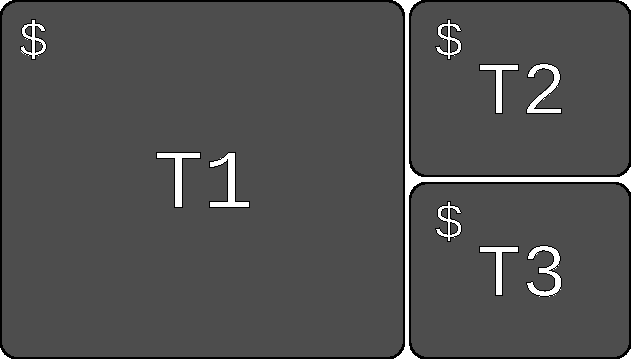
\includegraphics[scale=0.6]{images/terminals.pdf}}
		\caption{Figure 1: Disposition des terminals proposée.}
		\label{terminals}
	\end{figure}

Cette disposition vous permettra d'exécuter vos commandes \texttt{git} dans le terminal \texttt{T1}, tout en vous permettant d'exécuter des commandes de suivi dans les terminaux \texttt{T2} et \texttt{T3}.~\ref{terminals}\\

Dans un premier temps, positionnez \texttt{T1}, \texttt{T2} et \texttt{T3} dans le répertoire où vous allez travailler.\\

Ensuite, dans le terminal \texttt{T2} exécutez :
\begin{minted}[mathescape=true,escapeinside=||,tabsize=4
%	,fontsize=\footnotesize,
]{bash}
	watch -d -n3  'tree -a tpgit'
\end{minted}

Ensuite, dans le terminal \texttt{T3} exécutez :
\begin{minted}[mathescape=true,escapeinside=||,tabsize=4
%	,fontsize=\footnotesize,
]{bash}
	watch 'cat .gitconfig'
\end{minted}


%\hypertarget{objectifs}{%
\section{Objectifs}\label{objectifs}}

\begin{itemize}
\tightlist
\item
  Apprendre à se servir d'un Logiciel de Gestion de Version.
\item
  Matrisez le versionnement d'un projet logiciel.
\item
  Partager un projet et travailler en équipe.
\end{itemize}

\hypertarget{help}{%
\section{Help}\label{help}}

This text is \emph{emphasized with underscores}, and this is
\emph{emphasized with asterisks}.

This is \textbf{strong emphasis} and \textbf{with underscores}.

This is * not emphasized *, and *neither is this*.

feas\emph{ible}, not feas\emph{able}.

This \sout{is deleted text.}

H\textsubscript{2}O is a liquid. 2\textsuperscript{10} is 1024.

\emph{Italic} \ULforem \emph{Underline} \normalem

What is the difference between \mintinline[]{text}{>>=} and
\mintinline[]{text}{>>}?

Here is a literal backtick \mintinline[]{text}{`}.\\

This is a backslash followed by an asterisk: \mintinline[]{text}{\*}.\\

\textsc{Small caps}

\textsc{Small caps}

\textsc{Small caps}

\begin{minted}[]{java}
	if (a > 3) {
		moveShip(5 * gravity, DOWN);
	}
\end{minted}

\begin{minted}[]{haskell}
qsort []     = []
qsort (x:xs) = qsort (filter (< x) xs) ++ [x] ++
qsort (filter (>= x) xs)
\end{minted}

\leavevmode\hypertarget{special}{}%
Here is a paragraph.

And another.

\url{http://google.com}

\begin{figure}
\centering

\includegraphics{images/information.pdf}
\caption{This is the caption}
\end{figure}

\hypertarget{level-two}{%
\subsection{Level two}\label{level-two}}

\$-- An inline

\includegraphics[width=0.3125in,height=0.3125in]{images/information.pdf}
and a reference 
\includegraphics{images/information.pdf} with
attributes.\\

\begin{itemize}
\tightlist
\item
  line
\item
  line
\end{itemize}

and a reference 
\includegraphics{images/information.pdf} with
attributes.\\

\begin{minted}[]{java}
<div class="container">
    <div class="row">
        <div class="col-md-4">
			<img src="/img/wip3.jpg" alt="Work in progress"/>
		</div>
        <div class="col-md-7">
			<img src="/img/nslu2.jpg" alt="NSLU2.jpg"/>
        </div>
    </div>
</div>
\end{minted}

\begin{center}\rule{0.5\linewidth}{\linethickness}\end{center}

\begin{minted}[]{html}
<div class="row">
	<div class="col-md-4">
		<img src="/img/wip3.jpg" alt="Work in progress"/>
	</div>
	<div class="col-md-7">
		<img src="/img/nslu2.jpg" alt="NSLU2.jpg"/>
	</div>
</div>
\end{minted}

\hypertarget{howdie}{%
\subsection{Howdie}\label{howdie}}

It's easy to setup additional IP addresses on Debian Linux. This is
particularly useful for the NSLU which doesn't have a display so you
need to remotely connect to it.

Having more than one virtual network interface allows us to have both a
DHCP address and a static IP address, making the NSLU2 accessible
\texttt{pretty much always}.

\hypertarget{on-the-nslu}{%
\subsubsection{On the nslu}\label{on-the-nslu}}

I'm supposing you have somekind of IP address already setup. Also, you
should have a working DNS, although this shouldn't impact any of the
following.

Once you can ping the gateway machine, the gateway must be added so that
the nslu knows that he can attain addresses that are beyond his own
network.

Command is

\begin{minted}[]{bash}
	route add default gw 192.168.0.100
\end{minted}

Then the \mintinline[]{text}{/etc/resolv.conf} must be edited to the
same nameserver as the other box. Note that nslu should be able to ping
this nameserver once the gateway is setup.

For setting up the gateway we must enable ip forwarding:

\begin{minted}[]{bash}
echo 1 > /proc/sys/net/ipv4/ip_forward
\end{minted}

\hypertarget{additional-virtual-network-interface}{%
\subsubsection{Additional virtual network
interface}\label{additional-virtual-network-interface}}

If we want to setup alias cards, we can do something along the lines of

\begin{minted}[]{bash}
ifconfig eth0:N address    netmask
\end{minted}

However, it's probably easier to just edit the
\mintinline[]{text}{/etc/network/interfaces} file by adding something
like this

\{\% highlight bash\%\} iface eth0:0 inet static address 192.168.0.100
netmask 255.255.255.0 broadcast 192.168.0.255 network 192.168.0.0 pre-up
echo ``*** Starting eth0:0 alias ***" post-up echo ``*** Alias eth0:0
started ***" \#post-up route add -net 192.168.0.0 dev eth0 \#post-up
route add -host 192.168.0.10 dev eth0:1 \{\% endhighlight \%\}

This allows us to have a static IP address in addition to whatever other
configured addresses we might have. I used it to have both a DHCP
assigned address and a static local network address, allowing me to
always get access to the NSLU2, even if it's not getting an address
through DHCP.

Finally, must set up iptables to the correct rules!!!

I found and change a script to setup the tables to allow


%\paragraph{Avant de commencer}
%\begin{itemize}
%	\item Créer un répertoire TP2 dans votre répertoire de PA et y copier les fichiers \texttt{entiers.txt}, \texttt{annu.txt} et votre \texttt{.c} du TP précédent (renommez ce dernier en \texttt{tp2.c}).
%	\item Récupérer sur le compte de Walter Rudametkin, les fichiers \texttt{moyenne\_fichier.c} et \texttt{ldc.c} présents à l'adresse : \url{~wrudamet/public/IMA3/TP2/}
%\end{itemize}

\section{Initialisation de votre compte \texttt{git}}

Il est important de savoir qui a fait quoi. \texttt{git} a besoin d'une configuration pour votre.

Pour identifier vos futurs commits, tapez les commandes suivantes:

\begin{minted}[mathescape=true,escapeinside=||,tabsize=4
%	,fontsize=\footnotesize,
]{bash}
	git config --global user.name "votre nom"
	git config --global user.email nom.prenom@univ-lille1.fr
	git config --global core.editor kate
	git config --global push.default simple
\end{minted}


\section{Initialisation d'un dépôt \texttt{git}}





\subsection{Chargement à partir d'un fichier}


\begin{enumerate}
\item 
\item 
\end{enumerate}

\section{Questions s’il vous reste du temps}

\pagebreak

\section{Annexes}
\vspace{-0.5cm}
\begin{figure}[!h]
	\begin{minipage}[c]{0.40\textwidth}
		\centering
		\inputminted[
		%frame=lines,
		%framesep=2.5mm,
		%baselinestretch=0.8,
		fontsize=\small,
		linenos,
		tabsize=2,
		breaklines,
		xleftmargin=-25pt,
		numbersep=7pt,		
		%firstline=14,lastline=28
		%bgcolor=light-gray
		]
		{c}{\codes/ldc.c}
		\caption{\texttt{ldc.c}}
	\end{minipage}
	\hspace{0.1cm}
	\vrule{}
	\hspace{0.3cm}
	\begin{minipage}[c]{0.62\textwidth}
		%		\centering
		\inputminted[
		%frame=lines,
		%framesep=2.5mm,
		%baselinestretch=0.8,
		fontsize=\small,
		linenos,
		tabsize=4,
		breaklines,
		xleftmargin=4pt,
		numbersep=7pt,
		%		breaksymbolleft=,
		%firstline=14,lastline=28
		%bgcolor=light-gray
		]
		{c}{\codes/moyenne_fichier.c}
		\centering
		%		\captionof{listing}{entiers.txt}
		%		\captionsetup[justification=justified,singlelinecheck=false]
		%		\captionsetup{justification=raggedright, singlelinecheck=false}
		\caption{\texttt{moyenne\_fichier.c}}
	\end{minipage}
	%	\hspace{-1cm}
	%	\vrule{}
	%	\hspace{0.6cm}
	%	\begin{minipage}[b]{0.15\textwidth}
	%		\centering
	%		\inputminted[
	%		%frame=lines,
	%		%framesep=2.5mm,
	%		%baselinestretch=0.8,
	%		fontsize=\small,
	%		linenos,
	%		tabsize=2,
	%		%firstline=14,lastline=28
	%		%bgcolor=light-gray
	%		]
	%		{c}{\codes/moyenne_fichier.c}
	%		\captionsetup{justification=raggedright, singlelinecheck=false}
	%		\caption{annu.txt}
	%	\end{minipage}
	%	\captionof{listing}{SomeCaption}
	%	\label{lst:representation_examples}
\end{figure}
\end{document}